\section{Lancet Design}
\label{sec:design}
\label{sec:aet-model}
\system uses \emph{Causal Excision} to coordinate filesystem and
agent-context recovery through one rollback set $S$. Recovery starts with a
user report naming the files to roll back. The reference checkpoint denotes the state after a
selected call; the default is the committed boundary. The report identifies
a file-history range to withdraw, without identifying a faulty step or
deciding which edit was semantically wrong.

\begin{figure}[t]
\centering
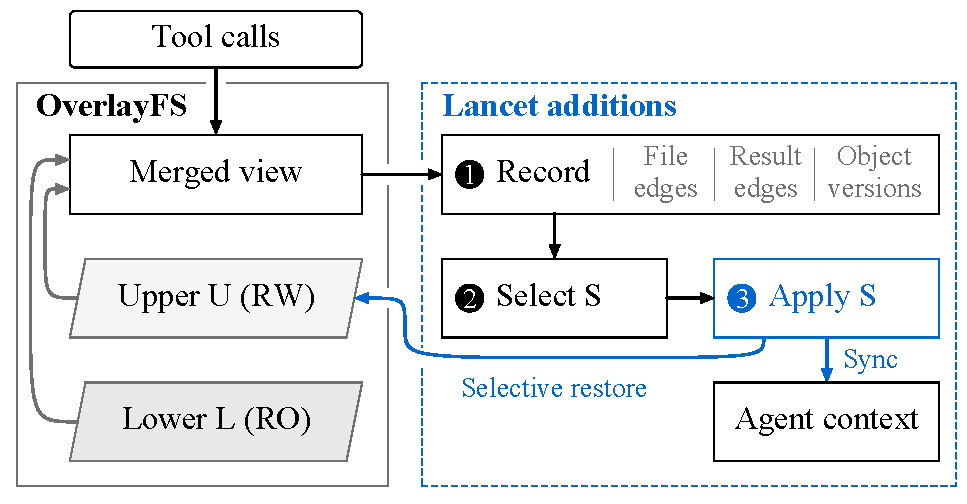
\includegraphics[width=\linewidth]{FIG-Lancet-Overview.pdf}
\caption{\textbf{Execution and selective recovery in \system.}
\small\emph{A user identifies the file to roll back. Shared call identifiers
connect dependency capture, saved
versions, and conversation records. The selected set $S$ drives both
filesystem restoration and agent-context updates.}}
\label{fig:overview}
\end{figure}

In Figure~\ref{fig:overview}, a persistent worker executes
calls in an OverlayFS merged view over a read-only lower baseline $L$ and
writable upper state $U$~\cite{overlayfs}. Tool-dispatch hooks integrate
SWE-agent and Codex; shared call identifiers link the file-effect ledger,
saved versions, and conversation log. The three challenges in
Section~\ref{sec:recovery-challenges} lead to three design points:
\begin{itemize}
\item \textbf{Select and validate $S$ via file and result dependencies.}
Start from the mutations of the reported files and audit their joint dependency
closure in an isolated branch (Section~\ref{sec:rollback-set}).
\item \textbf{Control filesystem recovery in user space.}
Retain object history incrementally, manage explicit OverlayFS checkpoints,
and restore affected objects alongside current independent updates
(Section~\ref{sec:userspace-fs}).
\item \textbf{Synchronize agent context via shared call identifiers.}
Use $S$ to remove withdrawn calls and results while preserving independent
observations within and across turns
(Section~\ref{sec:context-reconstruction}).
\end{itemize}

\subsection{Causal Excision}
\label{sec:rollback-set}
\label{sec:causal-excision}
Causal Excision withdraws selected mutations and their recorded dependent
effects while preserving independent work. It computes a rollback set $S$
through file and tool-result dependencies, validates the plan in an isolated
branch, and applies the same set to filesystem state and agent-visible
call/result pairs. Sections~\ref{sec:userspace-fs}
and~\ref{sec:context-reconstruction} describe how file restoration and
context synchronization apply this shared selection.

Figure~\ref{fig:dependency-closure} expands step 2 of
Figure~\ref{fig:overview}, using mutations of the reported file as the roots
of joint dependency closure.

\begin{figure}[t]
\centering
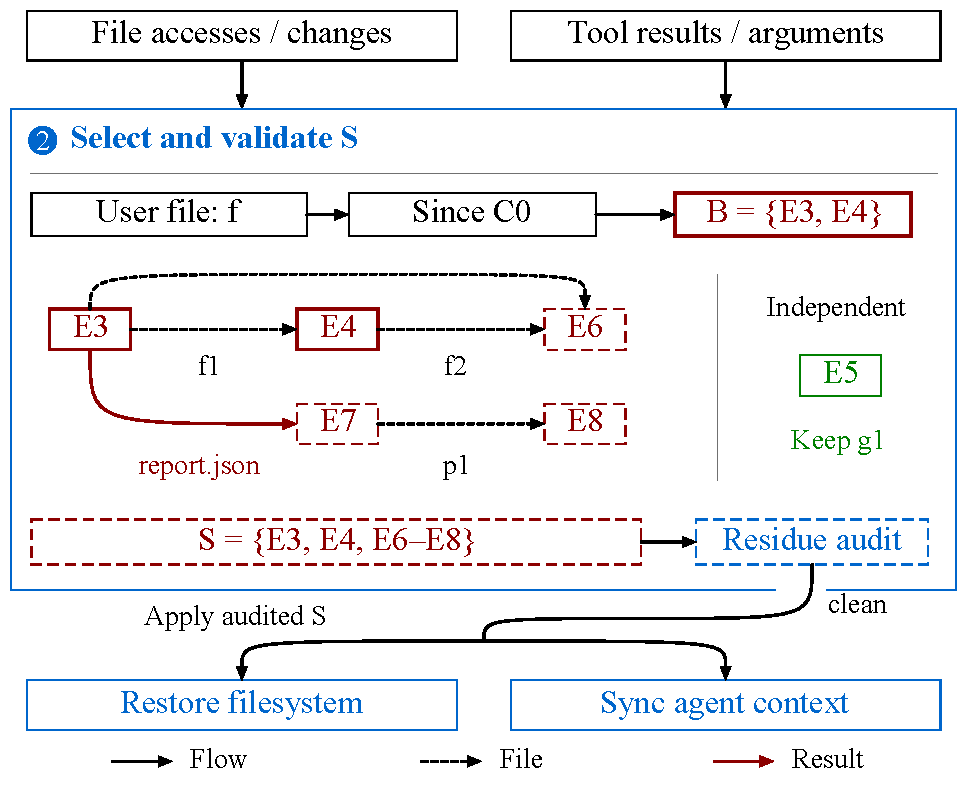
\includegraphics[width=\linewidth]{figures/design-workflow/Lancet-Dependency-Closure.pdf}
\caption{\textbf{Dependency capture and rollback-set selection.}
\small\emph{File and result records feed step 2 of Figure~\ref{fig:overview}.
The user names f with C0 before E3. Its mutations E3 and E4 seed joint
expansion to E3, E4, and E6--E8, preserving E5. A clean residue audit
supplies the same $S$ to filesystem and
agent-context recovery. Dashed black edges denote file dependencies;
red edges denote result reuse.}}
\label{fig:dependency-closure}
\end{figure}

\textbf{Capturing dependencies across both channels.}
Each exposed tool call receives an identifier linking its command, file
effects, version references, and call/result pair; a submitted script is
one recording unit. \texttt{strace}~\cite{strace} records reads and failed
lookups, while upper-state comparison identifies writes and deletions.
Table~\ref{tab:dependency-rules} gives the direct edges
$E_i\rightarrow E_j$ for $i<j$, where $R$, $W$, and $N$ denote reads or
access checks, mutations, and failed lookups. Related state includes path
hierarchies, resolved symlink ancestors, and cataloged object identifiers,
including known hard-link aliases; renames contribute both names.
The conversation log filters common and short strings from tool results
and matches distinctive values against later arguments to add result edges.

\begin{table}[!ht]
\centering
\caption{\textbf{Dependency rules between tool calls.}
\small\emph{For $i<j$, $\checkmark$ adds $E_i\rightarrow E_j$;
$\times$ means the pair alone adds no edge. File accesses refer to related state.}}
\label{tab:dependency-rules}
\footnotesize
\setlength{\tabcolsep}{2pt}
\renewcommand{\arraystretch}{1.12}
\begin{tabular*}{\linewidth}{@{\extracolsep{\fill}}lcc@{}}
\toprule
Relation & Access order & Edge \\
\midrule
Write--read (WR) & $W_i,\ R_j$ & $\checkmark$ \\
Write--write (WW) & $W_i,\ W_j$ & $\checkmark$ \\
Read--write (RW) & $R_i,\ W_j$ & $\times$ \\
Read--read (RR) & $R_i,\ R_j$ & $\times$ \\
Mutation--lookup & $W_i,\ N_j$ & $\checkmark$ \\
Lookup--write & $N_i,\ W_j$ & $\checkmark$ \\
\midrule
Result reuse & Result string in arguments & $\checkmark$ \\
\bottomrule
\end{tabular*}
\end{table}


\textbf{Selecting calls via joint dependency closure.}
The controller normalizes the reported paths, resolves known aliases, and
selects all active mutations of those files after the reference checkpoint
as roots $B$. It alternates forward expansion through file and result edges
until neither adds a call. In Figure~\ref{fig:dependency-closure}, a report
for f selects E3 and E4; file effects lead to E6, and reuse of the result from E3
leads to E7, whose output E8 reads. The resulting
$S=\{\mathrm{E3},\mathrm{E4},\mathrm{E6},\mathrm{E7},\mathrm{E8}\}$
preserves independent E5 and captures the chain across both graphs.
The controller derives one scope from the report; it does not enumerate
faulty-step candidates or use task-test success to choose where to stop.

\textbf{Checking recovery before model continuation.}
The filesystem controller supplies compatible pre-mutation versions for
overlapping paths written or deleted by $S$
(Section~\ref{sec:userspace-fs}). Before application, the runtime freezes
the graph, active call/result identifiers, and expected saved file entries.
It applies the plan in an isolated branch and checks for residual selected
calls, visible results, dangling dependencies, and mismatched file state.
Reported files must match the reference checkpoint; retained entries and
the lower baseline must remain unchanged. Missing history, incompatible
versions, or a failed check make recovery inconclusive. After a clean trial,
the runtime verifies that the history has not changed, applies the same
frozen plan, and repeats the audit before model continuation.
The official task verifier evaluates subsequent repairs separately.

\subsection{Filesystem Recovery via User-Space Control}
\label{sec:userspace-fs}
\label{sec:version-retention}
\label{sec:selective-reconstruction}
The selected calls can require a combination of file states absent from
every checkpoint. The user-space controller in \system translates $S$ into
object versions and restoration operations, using native Linux mount and
file interfaces. OverlayFS supplies the merged view and copy-on-write
behavior; the controller manages version history, checkpoint lifetimes,
and selective restoration.

\textbf{Retaining history via changed entries.}
Figure~\ref{fig:version-capture} separates incremental object history from
explicit checkpoints. Each logical recovery point references its parent
and records changed paths, contents, metadata, and deletion state;
unchanged state reuses its existing version. Immutable contents are shared
in the version store, while the active upper keeps separate writable
copies. E3 and E4 add f1 and f2; E5 adds g1 without copying earlier versions.
Recovery follows parent references to retrieve selected objects, applying
deltas where needed. A complete historical tree is materialized only when
requested, avoiding repeated directory cloning and a new mounted
checkpoint for every call.

\begin{figure}[t]
\centering
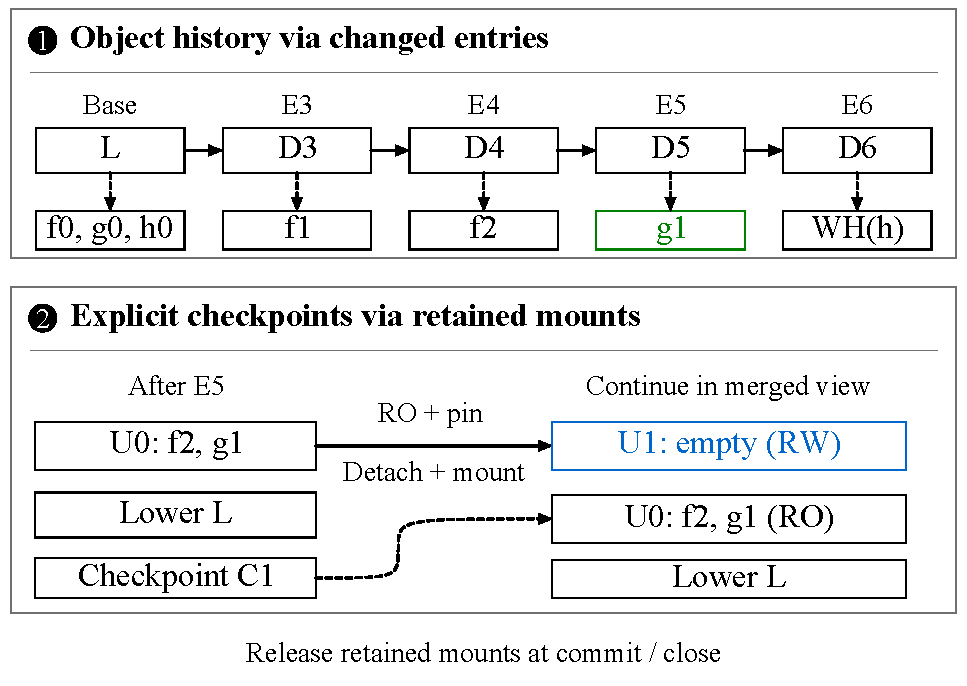
\includegraphics[width=\linewidth]{figures/design-workflow/Lancet-Version-Capture.pdf}
\caption{\textbf{Incremental history and explicit checkpoint creation.}
\small\emph{Changed entries extend object history. An explicit checkpoint
retains the old read-only view and starts a fresh writable upper; retained
mount references are released at commit or close. Solid arrows show flow;
dashed arrows associate saved file state with history records.}}
\label{fig:version-capture}
\end{figure}

\textbf{Managing checkpoints via retained mounts.}
For an explicit storage checkpoint, the caller quiesces writers. The
controller makes the current view read-only, retains a mount reference,
detaches the view, and mounts a fresh writable upper over the frozen layers.
In Figure~\ref{fig:version-capture}, checkpoint C1 references U0 and L
after E5, and execution continues in U1. Retaining the mount defers
superblock destruction to commit or close, while file data stay in their
existing layers. Section~\ref{sec:eval-file-commit} measures checkpoint
latency and the complete workflow, including reference release and cleanup.

\textbf{Reconstructing state via compatible object versions.}
The controller groups overlapping paths mutated by $S$, placing a selected
directory and its children together. For each group, it resolves the
nearest compatible saved state before its earliest selected mutation and
rejects retained mutations that overlap a group after its earliest selected
mutation. Earlier retained writes remain in the saved state of that group.
Groups may use different
historical versions; paths outside them retain their current state.
In Figure~\ref{fig:design-workflow}, f comes from V0 before E3, h from V1
before E6, and p from V2 before E7. V0 has correct f0 but predates g1;
V1 and V2 contain g1 together with affected f2. Selecting individual
entries preserves the required f0/g1 combination.

After isolated validation, the runtime checks the frozen history signature,
stops the worker, and applies the same $S$ and saved versions in the live
session. It restores the contents, metadata,
and deletion state of each group in the upperdir. Removing an upper entry
exposes its lower version or leaves the path absent. Removing f2 and the
whiteout hiding h therefore exposes f0 and h0; removing p1 makes p absent,
while independent g1 stays in $U$. The runtime refreshes mount scaffolding
and filesystem tracking without replaying retained commands, then applies
the same selection to agent context.

\subsection{Context Synchronization via Shared Call Identifiers}
\label{sec:context-reconstruction}
Recovery also removes observations of withdrawn effects
from the next model request. Shared identifiers let \system apply the same
$S$ to file-effect records and agent-visible call/result pairs, retaining
independent observations from partially withdrawn turns.

\begin{figure}[t]
\centering
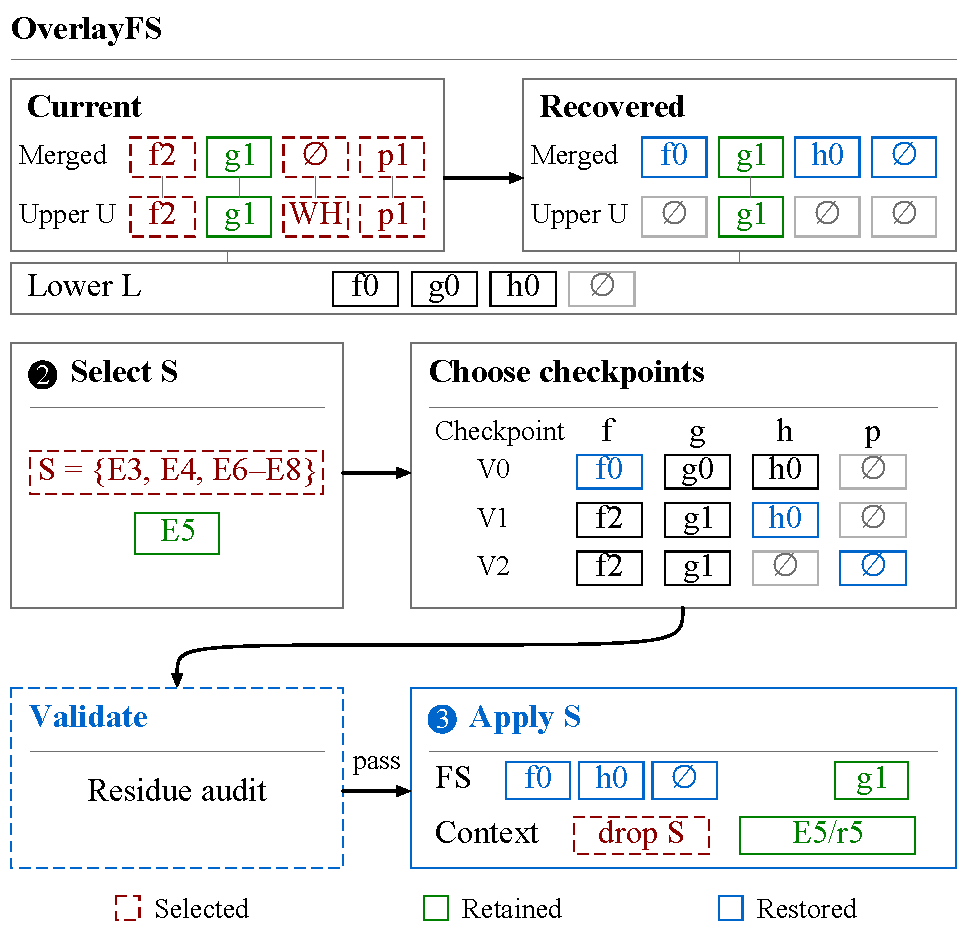
\includegraphics[width=\linewidth]{figures/design-workflow/Lancet-Design-Workflow.pdf}
\caption{\textbf{Applying one rollback set to files and agent context.}
\small\emph{Blue cells select saved states for f, h, and p over shared
lower $L$; current g1 remains active. The f0/g1 combination appears in no
saved row. The same $S$ removes selected context pairs and retains E5/r5.
The dashed frame denotes the isolated residue audit; WH is a whiteout and
$\varnothing$ denotes absence.}}
\label{fig:design-workflow}
\end{figure}

After restoration succeeds, selected ledger steps and their call/result
spans become inactive, with full records retained for audit. In the mixed
turn in Figure~\ref{fig:design-workflow}, withdrawing E6--E8 preserves
E5/r5, matching the retained g1 update. Turns with no surviving calls
are omitted. The native tool-call log filters assistant call lists and
their matching results; recovery removes stale control messages and adds
a notice describing retained and withdrawn effects.

System and task messages, surviving pairs, and the recovery notice form
the next model request. If older history is summarized to meet the context
budget, summaries are rebuilt from active spans so withdrawn results do
not reappear through compaction. Saving the ledger and conversation
together in session metadata keeps subsequent execution tied to the same
recovery decision.

\subsection{Correctness of Selective Recovery}
\label{sec:recovery-correctness}
Let $F$ be the normalized files named by the user, $c$ the reference
checkpoint, and $X_c$ its filesystem state. Let $H$ be the finite active
history, $G$ the union of recorded file and result edges, $W_i$ the mutation
footprint of $E_i$, and $V_i$ its pre-call saved versions. Write
$W(A)=\bigcup_{E_i\in A}W_i$. Edges point forward in call order. Footprints include
contents, supported metadata, deletions, related paths, and known aliases;
$\bowtie$ denotes footprint overlap. Calls execute serially over a fixed
lower baseline, with no untracked writers during recovery. Saved versions
faithfully represent this history, and file effects and call/result records
share identifiers. To cover actual propagation, $G$ must contain all true
dependencies within this managed state. State equality covers contents,
supported metadata, presence, and active call/result records.
Distinctive-string matching alone does not establish capture completeness.

Algorithm~\ref{alg:causal-rollback} formalizes Causal Excision by computing
the scope of the report and applying it. $\operatorname{Audit}$ checks
frozen expected versions, checkpoint
files, active identifiers, retained entries, and the lower baseline as
described in Section~\ref{sec:rollback-set}. Its acceptance condition is
independent of the test outcome for the original task.
Write $Z=(X,C,\operatorname{Active}(H))$. The fixed transformation $T_S$
restores each group from $V_{m(p)}$, projects records onto $R$, and marks
$S$ inactive. $\operatorname{Fresh}(A)$ checks the frozen history signature;
$\bot$ denotes rejection or inconclusive recovery.

\begin{algorithm}[H]
\caption{Causal Excision}
\label{alg:causal-rollback}
\footnotesize
\textbf{Input:} $F,c,H,G,V,Z$
\begin{enumerate}[label=\arabic*:,ref=\arabic*,leftmargin=1.7em,labelsep=.4em,topsep=2pt,itemsep=0pt,parsep=0pt]
\item $B\gets\{E_i\in H\mid i>c\ \land\ W_i\bowtie F\}$ \label{algline:file-roots}
\item \textbf{if} $B=\varnothing$ \textbf{return} $\bot$
\item $S\gets\operatorname{Reach}_G(B)$ \label{algline:closure-start}\label{algline:closure-end}
\item $R\gets H\setminus S$;
$\mathcal{P}\gets\operatorname{OverlapGroups}(W(S))$
\item $m(p)\gets\min\{i\mid E_i\in S,\ W_i\bowtie p\}$, $p\in\mathcal{P}$
\item \textbf{if} $\exists p\in\mathcal{P},E_j\in R:\ j>m(p)\land W_j\bowtie p$ \textbf{return} $\bot$ \label{algline:conflict}
\item $A\gets\operatorname{Freeze}(F,c,H,G,V,Z,S)$
\item $Z_t\gets T_S(\operatorname{Clone}(Z))$ \label{algline:restore}\label{algline:context}
\item \textbf{if} $\neg\operatorname{Audit}(Z_t,A)\lor\neg\operatorname{Fresh}(A)$ \textbf{return} $\bot$
\item $Z\gets T_S(Z)$
\item \textbf{return} $(Z,S,\operatorname{Audit}(Z,A))$
\end{enumerate}
\end{algorithm}

\textbf{Proposition 1 (file-scope rollback consistency).}
Under the assumptions above, an accepted recovery removes every call
reachable from $B$, preserves the retained history $R$, and satisfies
\[
  X^{+}|_F=X_c|_F,\qquad
  C^{+}=\operatorname{Project}(C,R).
\]
Filesystem state outside the restored groups is unchanged. Retained calls
have no dependency on the withdrawn scope in the covered dependency graph.

\emph{Proof by contradiction.}
Suppose recovery is accepted but violates the proposition. Then a dependency
is left unresolved, a filesystem entry is incorrect, or the active history
and context disagree with $R$.

Suppose a call depending on $B$ remains in $R$, or a retained call consumes
a withdrawn version or result. Capture completeness gives a path in $G$
from $S$ to that call. Its first edge leaving $S$ contradicts
$S=\operatorname{Reach}_G(B)$. Also, $T_S$ marks every call in $S$
inactive, so no selected call can remain active.

Suppose a filesystem entry is incorrect. Outside the restored groups,
$T_S$ makes no assignment, contradicting any change there. Within a group
$p$, faithful $V_{m(p)}|_p$ contains all earlier retained writes and no
selected mutation of $p$. A later retained mutation overlapping $p$ would
trigger rejection at line~\ref{algline:conflict}, contrary to acceptance.
Thus restoring $V_{m(p)}|_p$ cannot leave a selected effect or lose a
retained one; restoring one group cannot overwrite the restored state of a
disjoint group.
In particular, $X^{+}|_F\ne X_c|_F$ would require a surviving post-$c$
mutation of $F$ or an incorrect saved version. The former belongs to
$B\subseteq S$ and is removed; the latter contradicts faithful history.

Finally, suppose a withdrawn call/result remains visible or a retained pair
is lost. Shared identifiers and projection onto $R$ remove exactly $S$,
contradicting that discrepancy. The frozen-history check excludes a changed
plan between trial and application, and the final audit must pass before
continuation. Every possible violation therefore contradicts closure,
faithful restoration, projection, or acceptance.

\textbf{Corollary (idempotence of a fixed plan).}
Let $Z=(X,C,\operatorname{Active}(H))$ and let $T_S$ apply the frozen
saved versions, inactive marks, and record projection. Then
$T_S(T_S(Z))=T_S(Z)$.
\emph{Proof by contradiction.} Suppose a second application changes a
managed file entry, active mark, or call/result record. The first application
already assigns the fixed versions, marks $S$ inactive, and projects onto
$R$. Repeating those assignments cannot change an entry or mark, and
projecting records already in $R$ cannot change them. This contradicts the
assumed difference. Recovery notices and audit counters are outside this
state equality; the API rejects stale plans during application.

This proves consistency of the requested rollback, conditional on capture
coverage. It neither identifies an upstream mistake outside the reported
scope nor proves that the original task is solved. A semantically valid
checkpoint restores that validity for the reported files; subsequent task
completion is checked separately.

\subsection{Implementation}
\label{sec:implementation}
\system implements Causal Excision in a shared user-space controller,
decoupling recovery policy and agent-context synchronization from the
backing filesystem. The controller manages history, checkpoints, and
restoration through native Linux interfaces over OverlayFS.
Figure~\ref{fig:implementation} shows two implementations:
Ext4 uses ordinary file copying, while XFS uses reflink to share unchanged
data blocks between distinct versions. Support for additional backing
filesystems is concentrated in storage operations, allowing the dependency
graph, rollback selection, and agent integration to be reused.

\begin{figure}[t]
\centering
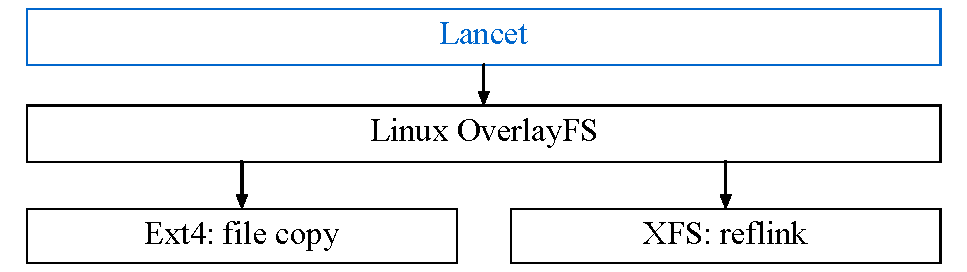
\includegraphics[width=\linewidth]{figures/design-workflow/Lancet-Implementation.pdf}
\caption{\textbf{Ext4 and XFS implementations.}
The Causal Excision controller shares recovery logic across two storage
backends.}
\label{fig:implementation}
\end{figure}
